\begin{enumerate}
\item The distance of the point $\brak{-3,4}$ from the $x-axis$ is
\begin{enumerate}
\item $3$ 
\item $-3$ 
\item $4$ 
\item $5$ 
\end{enumerate}
%vectors
\item In \figref{2012_v_fig1}, $P\brak{5,-3}$ and $Q\brak{3,y}$ are the points of trisection of the line segment joining $A\brak{7,-2}$ and $B\brak{1,-5}$.Then $y$ is equals
\begin{figure} [h]
\centering
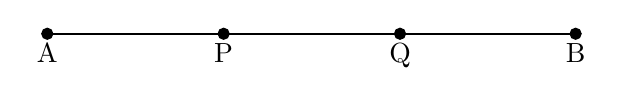
\begin{tikzpicture}[scale=1]
\draw[thick] 
    (-5.37, 4.92) --  % A
    (-3.13, 4.92) --  % P
    (-0.89, 4.92) --  % Q
    (1.34, 4.92) -- cycle;  % B
\node at (-5.37, 4.92) [below] {A};
\node at (-3.13, 4.92) [below] {P};
\node at (-0.89, 4.92) [below] {Q};
\node at (1.34, 4.92) [below] {B};
\filldraw 
    (-5.37, 4.92) circle (2pt)  % A
    (-3.13, 4.92) circle (2pt)  % P
    (-0.89, 4.92) circle (2pt)  % Q
    (1.34, 4.92) circle (2pt);  % B

\end{tikzpicture}
\caption{}
\label{2012_v_fig1}
\end{figure}
\begin{enumerate}
\item $2$ 
\item $4$ 
\item $-4$ 
\item $\dfrac{-5}{2}$ 
\end{enumerate}
\item The coordinates of the point $P$ dividing the line segment joining the points $A\brak{1,3}$ and $B\brak{4,6}$, in the ratio $2:1$ are:
\begin{enumerate}
\item $\brak{2,4}$ 
\item $\brak{3,5}$ 
\item $\brak{4,2}$ 
\item $\brak{5,3}$ 
\end{enumerate}
%circles
\item If the coordinates of one end of a diameter of a circle are $\brak{2,3}$ and the coordinates of its centre are $\brak{-2,5}$, then the coordinates of the other end of the diameter are:
\begin{enumerate}
\item $\brak{-6,7}$ 
\item $\brak{6,-7}$ 
\item $\brak{6,7}$ 
\item $\brak{-6,-7}$ 
\end{enumerate}
\item The area of a triangle whose vertices are $\brak{5,0}$, $\brak{8,0}$ and $\brak{8,4}$ $\brak{\text{in sq. units}}$ is
\begin{enumerate}
\item $20$ 
\item $12$ 
\item $6$ 
\item $16$ 
\end{enumerate}

\item If $A\brak{1,3}$, $B\brak{-1,2}$, $C\brak{2,5}$ and $D\brak{x,4}$ are the vertices of a parallelogram $ABCD$, then the value of $x$ is
\begin{enumerate}
\item $3$ 
\item $4$ 
\item $0$ 
\item $\dfrac{3}{2}$ 
\end{enumerate}
%vectors
\item Find the value of $k$, if the point $P\brak{2,4}$ is equidistant from the points $A\brak{5,k}$ and $B\brak{k,7}$. 
%vectors
\item Find the coordinates of a point $P$, which lies on the line segment joining the points $A\brak{-2,2}$ and $B\brak{2,-4}$ such that $AP = \dfrac{3}{7} AB$. 
%vectors

%vectors
\item If a point $A\brak{0,2}$ is equidistant from the points $B\brak{3,p}$ and $C\brak{p,5}$, then find the value of $p$. 
%vectors
\item A point $P$ divides the line segment joining the points $A\brak{3,-5}$ and $B\brak{-4,8}$ such that $\dfrac{AP}{PB} = \dfrac{K}{1}$. If $P$ lies on the line $x + y = 0$, then find the value of $K$. 
\item Find the ratio in which the line segment joining the points $\brak{1,-3}$ and $\brak{4,5}$ is divided by x-axis. 
\item Find the ratio in which the y-axis divides the line segment joining the points $\brak{5,-6}$ and $\brak{-1,-4}$. Also find the coordinates of the point of intersection. 

\item For what value of $k$, $\brak{ k > 0}$, s the area of the triangle with vertices $\brak{-2,5}$, $\brak{k,-4}$, and $\brak{2k+1,10}$ equal to $52$ sq. units? 

\item If the vertices of a triangle are $\brak{1,-3}$, $\brak{4,p}$ and $\brak{-9,7}$ and its area is $15$ sq. units, find the value$\brak{\text{s}}$ of $p$. 
\item Find the area of quadrilateral $ABCD$ whose vertices are $A\brak{-3,-1}$, $B\brak{-2,-4}$, $C\brak{4,-1}$ and $D\brak{3,4}$.

\item If the point $A\brak{x,y}$, $B\brak{3,6}$ and $C\brak{-3,4}$ are collinear, show that $x - 3y + 15 = 0$. 
\end{enumerate}
